\documentclass[10pt]{article}
\usepackage[utf8]{inputenc}
\usepackage{graphicx}
\usepackage{geometry}
 \geometry{
 a4paper,
 total={170mm,257mm},
 left=20mm,
 top=20mm,
 }
\usepackage{hyperref}
\usepackage{fontenc}
\usepackage{mathptmx}
\usepackage{geometry}
\usepackage{titling}
\usepackage{pgfplots}
\usepackage[demo]{graphicx}
\usepackage{subfig}
\setlength{\topskip}{0mm}
\setlength{\droptitle}{-8em} 
\title{{\large \textbf{CONCORDIA UNIVERSITY \\ DEPARTMENT OF COMPUTER SCIENCE AND SOFTWARE ENGINEERING \\ SOEN 6011: SOFTWARE ENGINEERING PROCESS: SUMMER 2019 \\ DELIVERABLE 1: OPEN PROBLEMS}}}
\author{\normalsize \textbf {STUDENT NAME: MANUSHREE MALLARAJU } \\ \normalsize \textbf{STUDENT IDENTIFICATION NUMBER: 40082236 }}
\date{}
\begin{document}
\maketitle
\section*{{\normalsize PROBLEM T1-OP5. Source(s): “Give a brief description, not exceeding one page, of your function, including the domain and co-domain of function, and the characteristics that make it unique. To ensure that you have attained sufficient background, Test 1 will have a problem related to your function.” }}

\section*{\normalsize \textbf{INTRODUCTION}}
\quad The exponential function \( ab^x \)is one of the power rules of math, which involves an exponent. This exponent is represented with a variable rather than a constant, and its base is represented with constant value rather than a variable. Let \( f(x) = ab^x \) be an exponential function where “b” is its change factor (or a constant), the exponent “x” is the independent variable (or input of the function), the coefficient “a” is called the initial value of the function (or the y-intercept), and “f(x)” represent the dependent variable (or output of the function)

\section*{\normalsize \textbf{DOMAIN:}}
\quad The domain is a set of all real numbers,R. where :\( b > 0 \) ,\( x > 0 \)

\section*{\normalsize \textbf{CO DOMAIN}}
\quad The co-domain is also a set of all real numbers, R.

\section*{\normalsize \textbf{CHARACTERISTICS}}
Fig:1 Exponential functions defined by an equation of the form $ab^x$ are called exponential decay functions if the change factor “b” (fixed base value) is \( 0<b<1 \), or it is also called exponential growth functions if the change factor is \( b > 0 \) \newline
Fig:2 The y-intercept is (0,a) and it is located at the initial value “a”. There is no x-intercept. The domain for an exponential decay function of this form is all real numbers and the range is \( y > 0 \)
\section*{\normalsize \textbf{GRAPH}}
\begin{figure}
    \centering
    \subfloat[Exponential Decay]{{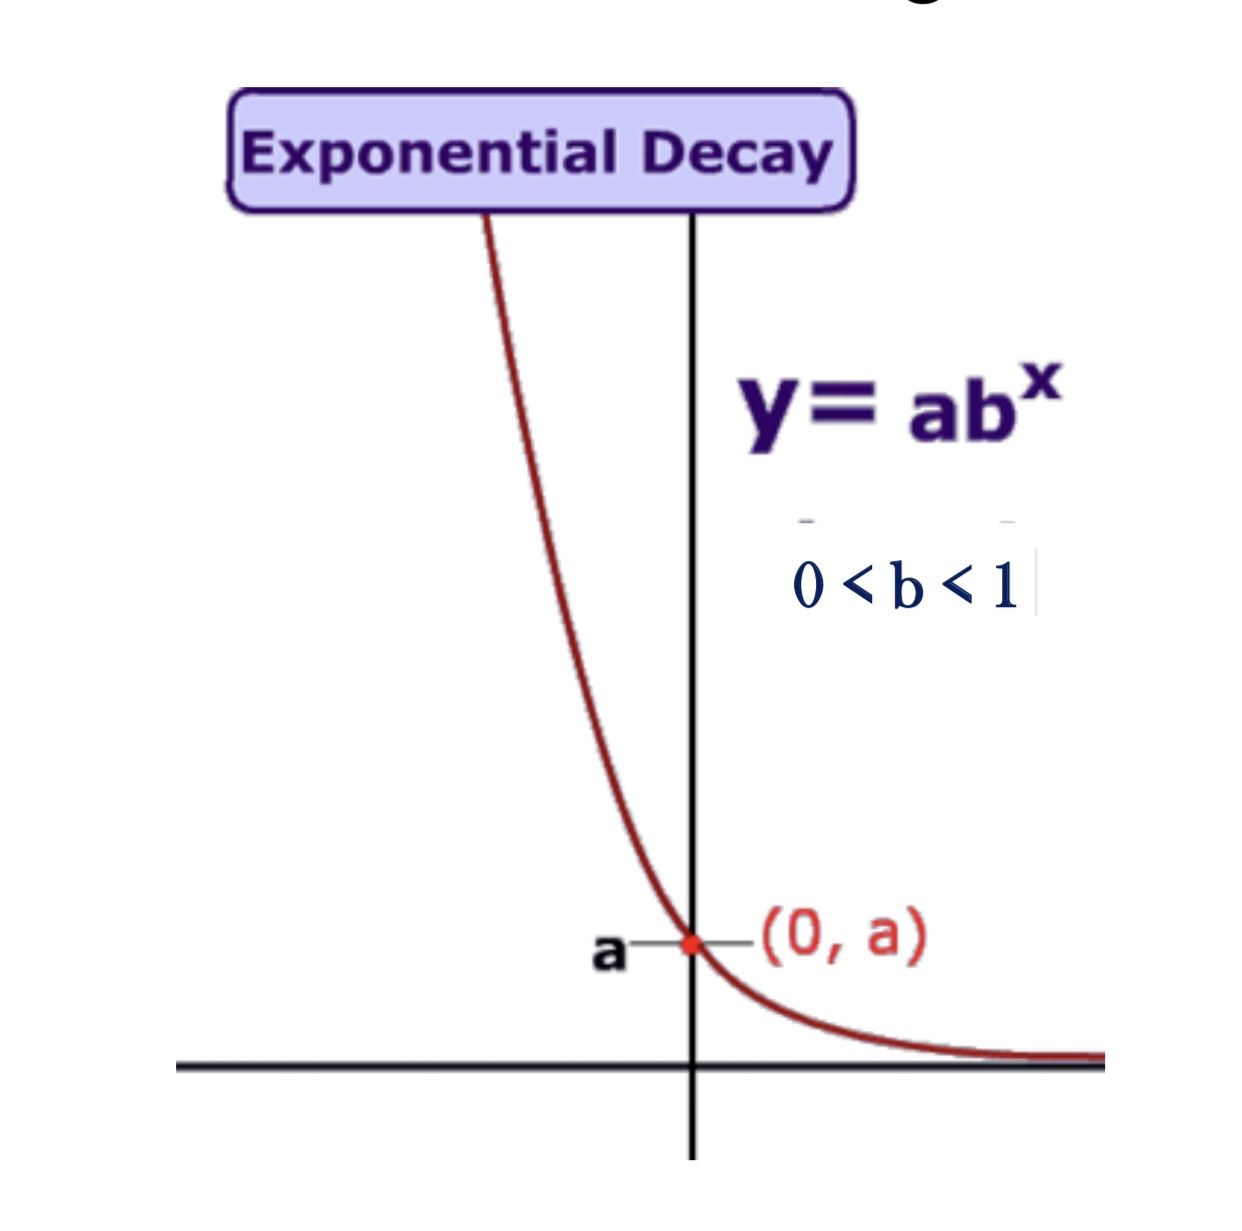
\includegraphics[width=5cm]{Function6/IMG_1640.jpg} }}
    \qquad
    \subfloat[Exponential Growth]{{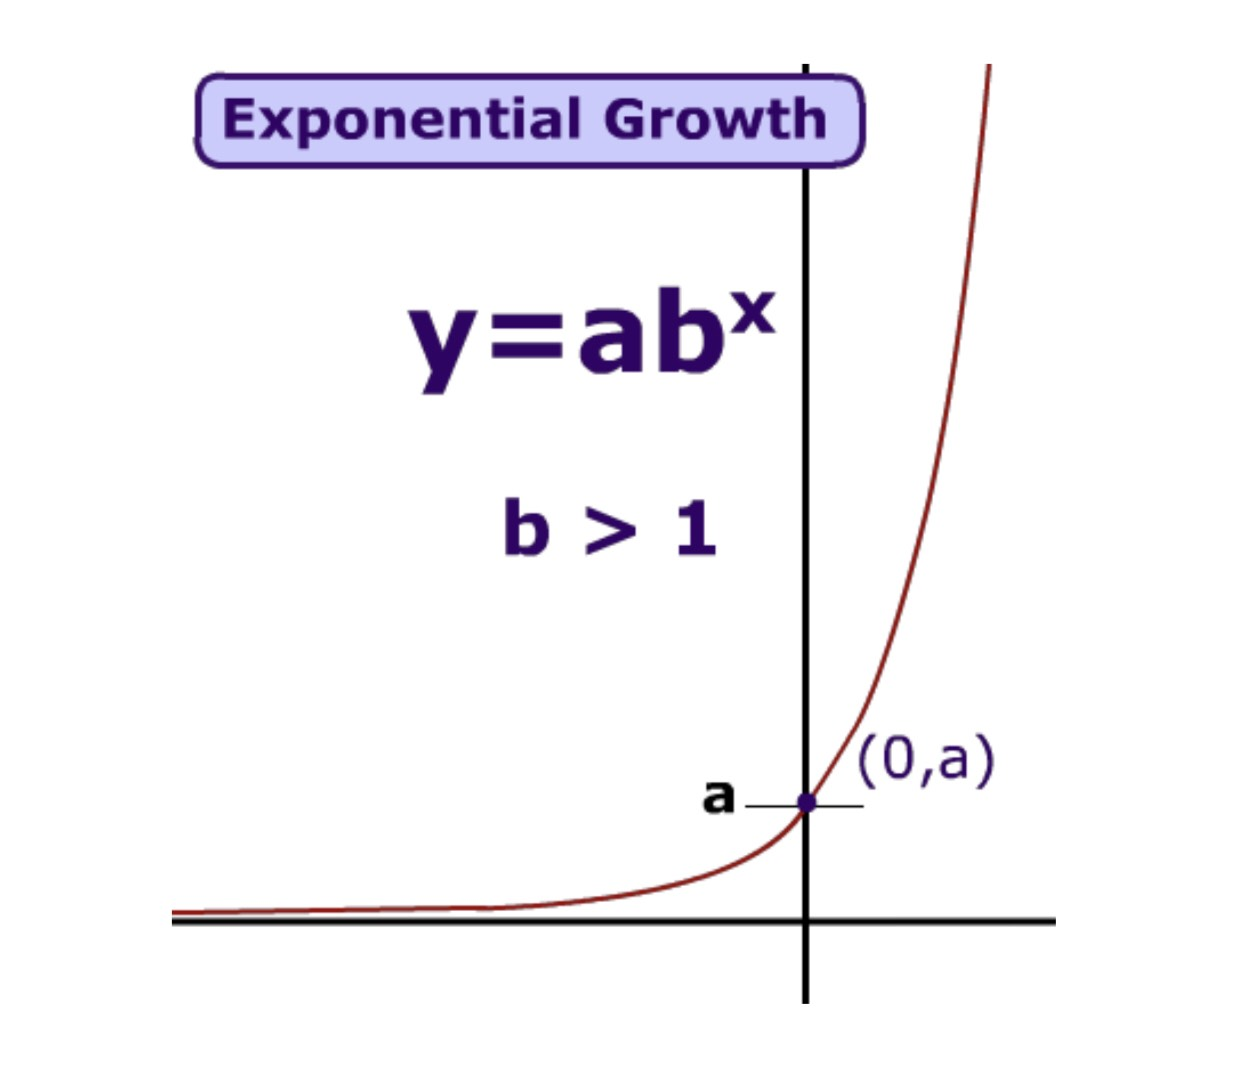
\includegraphics[width=5cm]{Function6/IMG_1641.jpg} }}
    \caption{Representation of $ab^x$ }
\end{figure}
\\
\\
\\
\pagebreak
\section*{{\normalsize PROBLEM 2: Source(s): “Express requirements of your function based on the style given in the ISO/IEC/IEEE
29148 Standard. Associate each requirement with a unique identifier. Make any assumptions explicit. ” }}
\section*{Requirements:}
\section*{1:}
\begin{itemize}
  \item ID			:FR-1
  \item TYPE		:Functional Requirement
  \item DIFFICULTY	:Easy
  \item VERSION		:1.0
  \item DESCRIPTION	: •	When  a = 0  or  b = 0  the function shell simplify to  y = f(x) = 0, so all the values should be greater than 1.
\end{itemize}
\section*{2:}
\begin{itemize}
  \item ID			:FR-2
  \item TYPE		:Functional Requirement
  \item DIFFICULTY	:Easy
  \item VERSION		:1.0
  \item DESCRIPTION	: When  b = 1  the function shell simplify to  y = f(x) = a,  so all the values of b should be greater than 1.

\end{itemize}

\section*{3:}
\begin{itemize}
  \item ID			:FR-3
  \item TYPE		:Functional Requirement
  \item DIFFICULTY	:Easy
  \item VERSION		:1.0
  \item DESCRIPTION	:Expressions with negative bases such as $(–3)^3/2$  or  $(–1.4)^2/5$ result in undefined values, the base b in an exponential function must be positive. 
\end{itemize}
\section*{{\normalsize EXPLICIT ASSUMPTIONS}}
1. 'a' is a constant which can be the combinations of positive or negative numbers.\\
\\
2. 'b' is a constant which can be the combinations of positive  number.\\\\
3. 'x' is a variable and a real number which values can be in the range between -39 to +39.
\pagebreak


\section*{{\normalsize PROBLEM 3: Source(s): “Collaboratively brainstorm and mind map with your team members to decide a pseudocode format. The pseudocode format must be identical across the team. Select algorithms for implementing your function and all its subordinate functions, if any.
Give technical reasons for selecting each of the algorithms, including their advantages and disadvantages. (This, by reference, means that you must have at least two options to choose from.)
Give a brief description of your algorithms and express each of them in pseudocode.” }}

\section*{{\normalsize There are several ways to implement the function $ab^x$.}}
\quad1. Iteartive Algorithm\\
\quad2. Recursive Algorithm\\
\quad3. Divide and Conquer Algorithm\\
\quad \quadand so on..


\section*{\normalsize \textbf{1. Algorithmic Paradigm: ITERATIVE .}}
\quad \quad An Iterative algorithm is an approach which executes the steps in number of iterations, using the looping construct.\\
\quad Iterative algorithm uses looping statements such as: for loop, while loop or do-while loop to re-execute the same statements.

\textbf{Advantages :}\\
- Iterative algorithm is faster to implement, since it uses looping structure.\\
- Tracing of Iterative algorithm is very easy.\\
- Iterative algorithm is more efficient with respect to time and space.\\

\textbf{Disadvantages :}\\
- Once the condition fails, Iteration terminates the execution of the program.
- Iterative solution are high efficient in terms of time and space.



\section*{\normalsize \textbf{2. Algorithmic Paradigm: RECURSIVE  .}}\\
\quad A Recursive algorithm is a type of implantation approach in which a function calls by itself during the execution of the program, until the base conditions are met.


\textbf{Advantages :}\\

- Recursive algorithm reduces unnecessary calling of function.\\
- Recursive algorithm helps to solve many problems easily.

\textbf{Disdvantages: }\\

- Understanding of the code in recursive functions is very confusing.\\
- Since the function calls itself in Recursive, it will be difficult to debug the code.\\
- In Recursive algorithm, its mandatory to use control statements like if, to return some value from the function.\\
- Recursive algorithm takes more processor time or memory.\\

\section*{\normalsize \textbf{Reason for selecting ITERATIVE ALGORITHM over RECURSIVE ALGORITHM .}}\\

\quad \quad  * Using Iterative algorithm is it easy to understand the flow of the program, where each step of the iteration is very clear.Whereas with Recursive, since the function calls itself, it is diffult to understand the flow of the program\\

\quad* Iterative algorithm using looping structure which is comfortable to trace the program, whereas Recursive Algorithm using branching structure.\\

\quad* If the base conditions are not met, Recursive algorithms have bad performances which leads to infinite call of its own function. Whereas in Iterative, the flow of the program can be easily debugged.
\pagebreak

\section*{\normalsize \textbf{Psuedocode using ITERATIVE ALGORITHM .}}\\
Function to calculate power using {\normalsize Newton's method of Nth root}\\
\\
 Nth root function

 \textbf{Power function:}\\
 1.Input : Base, Exponent\\
 2. \quad \textbf{if} Exponent > 0\\
 3.   \quad \quad \textbf{while} (Int of Exponent > 0)\\
 4.       \quad\quad\quad  result = result * base\\
 5. 		\quad\quad\quad Exponent = Exponent -1\\
 6.    \quad \quad end while\\
 7. \quad else\\
 8. 	\quad \quad  \textbf{while} (Int of Exponent < 0)\\
 9.     \quad \quad \quad result = result * base\\
 10. 	\quad \quad \quad Exponent = Exponent + 1\\
 11.  \quad \quad  end while\\
 12.\quad \quad return result\\
 13. \quad end if
  \\
  \\
 \textbf{nRoot function:}\\
 1. \quad Input: Value, Nthroot\\
 2. \quad ranVal = 4, precision = 0.0001, x = 1, dx = 2147483647\\
 3.\quad \textbf{while}(dx > precision)\\
 4. \quad \quad    x = ((N - 1.0)*ranVal + A/power(ranVal,N-1))/N\\
 5 	\quad \quad dx = x - ranVal\\
 6.\quad \quad	\textbf{if} (dx <0)\\
 7 	  \quad \quad \quad   dx = dx*-1\\
 8 \quad \quad 	precision = x\\
 9. \quad end while\\
 10. \quad return x\\
 

\bibliography{reference.bib}
\bibliographystyle{plain}
\nocite{Manushree:2019}\\
\bibliographystyle{plain}
\nocite{Manushree1:2019}
\bibliographystyle{plain}
\nocite{Manushree2:2019}
\bibliographystyle{plain}
\nocite{Manushree3:2019}
\bibliographystyle{plain}
\nocite{Manushree4:2019}
\bibliographystyle{plain}
\nocite{Manushree5:2019}
\bibliographystyle{plain}
\nocite{Manushree6:2019}
\bibliographystyle{plain}
\nocite{Manushree7:2019}
\bibliographystyle{plain}
\nocite{Manushree8:2019}
\bibliographystyle{plain}
\nocite{Manushree9:2019}
\bibliographystyle{plain}
\end{document}